\documentclass{article}
\title{高校数学やり直し II — 三角関数・図形と方程式・ベクトル}
\author{TeX 図書館}

\begin{document}

\section{読み方 — 前作とのつながりと 3 つの道具}

前作(高校数学やり直し)は二次関数・三角比・指数対数・数列をやり直しました。その後、大学数学入門へつながる一本道ができています。しかし、その道の中間には\textbf{橋が 2 か所}かかっていませんでした。1 つは\textbf{三角関数}(三角比を一般の角に広げて、波として扱えるようにする話)、もう 1 つは\textbf{ベクトル}(幾何を計算に翻訳する話)です。この本は、その 2 本の橋と、その間の\textbf{図形と方程式}(座標平面で図形を式にする話)を埋めます。

つまずきの原因は、前作と同じく 1 か所です。\textbf{「数と図形の往復」ができないまま、式変形だけを追う}こと。三角関数は単位円という図の上で見ると形が全部読め、ベクトルは矢印の絵がそのまま計算の意味になります。絵を先に描き、式を後から載せる方針は変えません。

\subsection{全 10 節の見取り図}

節の配分は次のとおりです。

\begin{enumerate}
\item 第 1 節: 読み方。方針と道具を決めます。
\item 第 2〜4 節: 一般角・三角関数・加法定理。三角比を波の数学へ広げます。
\item 第 5〜6 節: 図形と方程式。直線と円を式にします。
\item 第 7〜9 節: ベクトル。矢印の足し算から内積まで。
\item 第 10 節: まとめと次の一歩。
\end{enumerate}

各節の終わりには\textbf{解答の指針}を置きます。まず自力で 5 分考えてから、その欄を開いてください。

\subsection{本書で最初に使う式は 2 つだけ}

道具は次の 2 つに絞ります。1 つめは、半径 1 の円(単位円)を使った三角関数の定義です。角 \( \theta \) の点 \( (\cos\theta, \sin\theta) \) が円の上を回る、という 1 行がすべての出発点です。

\[ (\cos\theta, \sin\theta) \quad \text{on } x^{2} + y^{2} = 1 \]

2 つめは、ベクトルの\textbf{内積}です。2 つのベクトルの「似ている向き」を 1 つの数にしたもので、第 8 節で詳しくやります。

\[ \vec{a} \cdot \vec{b} = |\vec{a}| |\vec{b}| \cos\theta \]

\begin{quote}
\textbf{【注意】}\ 三角比と三角関数の違いを混同しないこと。三角比は「直角三角形の辺の比」で、角は 0 度から 90 度までしかありません。三角関数は\textbf{任意の角}に広げたもので、回転の数学です。波・円運動・振動はすべて三角関数の領域で、三角比の延長として計算できます。
\end{quote}

\textbf{解答の指針:}\ まず問題が「図形の話か、波の話か、向きの話か」を見分ける。図形なら第 5〜6 節の式、波なら単位円の回転(第 2〜3 節)、向きならベクトル(第 7〜9 節)の道具を使います。どれも最後は\textbf{図を描いてから式を立てる}のが共通の手順です。絵を描かずに式だけ追うと、符号と向きのミスが必ず出ます。

\section{一般角と弧度法 — 角を広げて、弧で測る}

三角比では角は 0 度から 90 度まででした。しかし回転はもっと自由です。\textbf{好きなだけ回転できる角}を\textbf{一般角}と呼びます。時計の針を 1 周まわすと 360 度に戻りますが、途中のどこでも「角」として意味がある、という見方が一般角です。

\subsection{回転の向きと符号}

数学では\textbf{反時計まわりを正、時計まわりを負}と決めます。−30 度は「時計まわりに 30 度」で、360 度回ると元の位置。つまり \( -30 \) 度と \( 330 \) 度は\textbf{同じ向き}を指します。一般角では「同じ向きの角は無数にある」(\( \theta \) と \( \theta + 360k \) 度)ことが重要で、これが第 3 節の「波が繰り返す」性質の元になります。

\subsection{弧度法: 角度を「弧の長さ」で測る}

単位円(半径 1)の中心から角 \( \theta \) を開くと、円周に沿った弧の長さが決まります。\textbf{この弧の長さをそのまま角の大きさ}とするのが\textbf{弧度法}です。1 周は半径 1 の円の円周 \( 2\pi \) なので、360 度 = \( 2\pi \) ラジアン、180 度 = \( \pi \) ラジアン、90 度 = \( \pi/2 \) ラジアンです。

なぜ度でなくラジアンを使うのか。ラジアンなら「角」がそのまま「弧の長さ」として現れるので、\textbf{微分したときの式がきれいになる}からです(大学数学入門で \( (\sin x)' = \cos x \) となるのはラジアンだから)。物理の波や振動もラジアンで書きます。換算は 1 つ覚えれば十分です。

\[ 180^{\circ} = \pi \ \mathrm{rad} \]

\begin{figure}
\centering
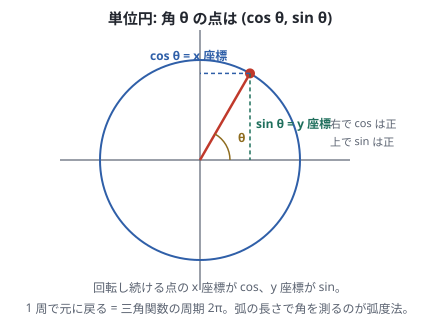
\includegraphics[width=0.85\textwidth]{figures/unit-circle.svg}
\caption{単位円と一般角: 円上の点が (\(\cos\theta\), \(\sin\theta\))}
\end{figure}

\begin{quote}
\textbf{【注意】}\ 弧度法のラジアンは「単位」ではなく「無名数」です。\( \pi/2 \) は「約 1.57(弧の長さ)」という数そのものです。「1.57 rad」と書くことはあっても、単位変換の感覚は「度 = \( \pi \) ラジアンに対応する表」という表で処理します。
\end{quote}

\textbf{解答の指針:}\ 一般角の問題では、(1) まず角を「基準の角 + \( 360k \) 度(または \( 2k\pi \))」の形に書く、(2) 基準の角が 0〜90 度なら前作の三角比の表がそのまま使える、(3) 象限(どの区画か)で符号が決まる(cos は右で正、sin は上で正)と確認する。ラジアン↔度の換算は 180 = \( \pi \) を掛けるだけ。単位円の絵を描けば、符号ミスはほぼなくなります。

\section{三角関数 — グラフと周期性}

単位円上の点 \( (\cos\theta, \sin\theta) \) は、角が回ると円の上を回り続けます。この点の y 座標が sin、x 座標が cos です。\textbf{角を横軸に、座標を縦軸にプロットすると、波が出る}。これが三角関数のグラフです。

\subsection{sin と cos は同じ波}

sin のグラフは 0 から始まる波、cos のグラフは 1 から始まる波で、\textbf{形はまったく同じで、横に \( \pi/2 \) ずれた}だけです。周期は \( 2\pi \)(1 周で元に戻る)。振幅は 1(最高 1、最低 -1)。

\[ y = \sin\theta \qquad y = \cos\theta \]

この「回転が波を作る」見方の応用は幅広い。音は空気の振動(sin の形)、交流電気は電圧の振動、腕時計の振り子も同じ。第 7 節の物理本(波)と直接つながるのはここです。振幅・周期・位相(波の始まりの位置)の 3 つのつまみを動かすと、どんな波も作れます。

\[ y = A \sin(b\theta + c) \]

振幅 \( A \)、周期は \( 2\pi/b \)、始まりは \( c \) でずれる、と読みます。

\begin{figure}
\centering
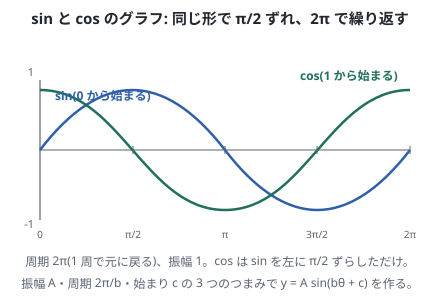
\includegraphics[width=0.9\textwidth]{figures/trig-graph.svg}
\caption{sin と cos のグラフ: 同じ形で \( \pi/2 \) ずれ、\( 2\pi \) で繰り返す}
\end{figure}

\subsection{tan は「傾き」の関数}

tan \( \theta \) は「原点から円上の点を結ぶ直線の傾き」です。つまり tan は\textbf{斜めの直線がどれだけ急か}を表す数。傾きは垂直になると急に行き止まり(無限大)になるので、tan のグラフは \( \pi/2 \) ごとに飛びます。実際の計算では、tan は sin ÷ cos として処理するのが安全です。

\begin{quote}
\textbf{【注意】}\ \( \sin^{2}\theta + \cos^{2}\theta = 1 \) は最もよく使う恒等式です。単位円では「点は半径 1 の円上にある」ことそのものであり、覚えるというより\textbf{絵から読み取る}式です。平方完成と同じく、式を変形する道具として頻出します。
\end{quote}

\textbf{解答の指針:}\ 三角関数の問題では、(1) 単位円またはグラフを描く、(2) 求めたい値が y 座標(sin)、x 座標(cos)、傾き(tan)のどれかを判定する、(3) 周期 \( 2\pi \) を使って角を 0〜\( 2\pi \) の範囲に折り返す。方程式を解くときは「円上の点が 2 つある」のが普通の答えの形です(第 1 象限と第 2 象限など)。グラフを描かずに解を 1 つで済ませてしまうのが最大のミスです。

\section{加法定理 — 和の公式で組み立てる}

「\( \sin(30^{\circ} + 45^{\circ}) = \sin 30^{\circ} + \sin 45^{\circ} \)」は\textbf{間違い}です。和の三角関数は、和の三角関数ではありません。正しい組み立て方を与えるのが\textbf{加法定理}です。

\[ \sin(\alpha + \beta) = \sin\alpha\cos\beta + \cos\alpha\sin\beta \]
\[ \cos(\alpha + \beta) = \cos\alpha\cos\beta - \sin\alpha\sin\beta \]

\subsection{なぜ掛け算の形になるのか}

直感の説明は、\textbf{「回転を 2 回掛ける」から}です。角 \( \alpha \) と角 \( \beta \) を続けて回すことは、角 \( \alpha + \beta \) の回転と同じ。しかし「x 座標と y 座標を混ぜて回す」操作なので、結果の座標は\textbf{sin と cos の掛け算の組み合わせ}で書けるしかない。加法定理は「2 回の回転を 1 回にまとめる」式であり、この構造は行列(大学数学入門)と同じ形をしています。

\subsection{加法定理から出てくる便利な道具}

加法定理は、覚える量を減らす発電所です。倍角の公式(\( \sin 2\theta = 2\sin\theta\cos\theta \))は \( \beta = \theta \) を代入しただけ。半角の公式や積和の公式も、すべてここから導けます。\textbf{全部暗えるのではなく、加法定理 2 本と、導き方の方向だけ覚える}のが高校数学のやり直しの正解です。

実用上の意味も押さえます。音の重ね合わせで、近い周波数の 2 つの波の和は「ゆっくり脈打つ 1 つの波」に書き換えられます(うなり)。これは積和の公式そのもので、フーリエ解析入門(音の分解)への入口です。式の形と現象の名前が結びつくと、三角関数は「暗記」から「道具」に変わります。

\begin{quote}
\textbf{【注意】}\ 加法定理の符号ミスは定番のミスです。\( \cos(\alpha - \beta) = \cos\alpha\cos\beta + \sin\alpha\sin\beta \) のように、引いたときに cos の式では符号が変わる(足し算になる)のは、cos が偶関数(\( \cos(-\theta) = \cos\theta \))だから。符号の理由まで説明できない場合は、\( \beta = -\beta \) を代入して確認する癖をつけてください。
\end{quote}

\textbf{解答の指針:}\ 加法定理の問題では、(1) 与えられた角を「既知の角の和・差」に分解する(75 度 = 45 + 30)、(2) どの定理(sin の和か cos の和か)を使うかを書く、(3) 代入して整理する。逆方向(和を角度に戻す)の問題では、式を定理の形に「組み立て直す」のが手順です。2 倍角は \( \beta = \theta \) の特殊形だと意識して、公式の暗記量を増やさないことが続けるコツです。

\section{図形と方程式 — 直線を式にする}

ここから場面を、波の世界から座標平面の世界へ移します。\textbf{図形と方程式}は、その名のとおり「図形を方程式に翻訳する」話です。点が動いて描く軌跡を、x と y の条件式として書けば、図形の問題が式変形の問題になります。

\subsection{直線: 条件を式に書く}

点 \( (x_{1}, y_{1}) \) を通り、傾き \( m \) の直線は次の式で書けます。

\[ y - y_{1} = m(x - x_{1}) \]

読み方は「y が y1 からどれだけ動いたかは、x が x1 からどれだけ動いたかの m 倍」。傾き \( m \) は\textbf{x が 1 増えると y が m 増える}という変化率で、中学の一次関数と同じものです。2 点を通る直線なら、傾きをまず計算し、その傾きと 1 点から上の式を作ります。

平行と垂直が式でどう書けるかも押さえます。\textbf{平行は傾きが等しい}(\( m = m' \))。そして\textbf{垂直は傾きの積が -1}(\( mm' = -1 \))。垂直の条件は覚えるしかありませんが、絵で確認するなら「x 軸に近い直線と y 軸に近い直線は垂直になる」ことを手で描いてみると納得できます。

\subsection{距離: 式で測る}

2 点 \( (x_{1}, y_{1}) \), \( (x_{2}, y_{2}) \) 間の距離は、三平方の定理(ピタゴラスの定理)を式にしたものです。

\[ d = \sqrt{(x_{2} - x_{1})^{2} + (y_{2} - y_{1})^{2}} \]

読み方は「x 方向の差と y 方向の差で直角三角形を作り、斜辺が距離」。この式はベクトル(第 8 節)でも同じ形で出てきます。\textbf{距離の式は、三平方の定理の座標版}と覚えると、暗記が理解に変わります。

\begin{quote}
\textbf{【注意】}\ 「直線の式を立てる」問題で最も多いミスは、傾きと通る点を取り違えることです。式を立てる前に「傾きは何か、通る点はどこか」を 2 行で書き出す。傾きが分からない問題でも、平行・垂直の条件から傾きが先に決まることが多いので、傾きを最初の目標にします。
\end{quote}

\textbf{解答の指針:}\ 直線の問題では、(1) 傾きを確定する(与えられるか、平行・垂直から出す)、(2) 通る点とセットで式を立てる、(3) 図を描いて符号と位置を確認する。交点は連立方程式、距離は三平方の式、と道具を割り当てます。図形の問題を式に翻訳するときは、最後に必ず図で答えの位置を確認するのが、翻訳ミスを防ぐ手順です。

\section{円の方程式 — 中心と半径を式にする}

円は「中心からの距離が一定の点の集まり」です。この言葉を距離の式に代入すると、円の方程式がそのまま出ます。

\[ (x - a)^{2} + (y - b)^{2} = r^{2} \]

中心 \( (a, b) \)、半径 \( r \) の円です。読み方の核心は\textbf{「x から a を引く = 点を右に a 動かす」}という符号の対応。中心 (2, 3) なら x - 2, y - 3 になります。式の左辺は三平方の定理そのもので、x 方向の差の 2 乗と y 方向の差の 2 乗の和が、半径の 2 乗に等しい、という意味です。

\subsection{一般形から標準形へ: 平方完成が再登場}

展開された式(\( x^{2} + y^{2} + 4x - 6y + 9 = 0 \) のような形)を与えられたら、\textbf{平方完成}で標準形に戻します。前作で二次関数の平方完成を練習したのは、ここで回収されます。x の項と y の項をそれぞれまとめ、平方完成すれば中心と半径が読み取れます。

\subsection{円と直線: 共有点の数は方程式の解}

円と直線が交わるかどうかは、\textbf{連立方程式の解の個数}の問題に翻訳されます。円の方程式に直線の式を代入すると 2 次方程式になるので、判別式(D)の符号が「2 点で交わる / 1 点で接する / 交わらない」に対応します。\textbf{接する = 解がちょうど 1 つ}。この「図形の話を方程式の個数に翻訳する」発想が、この分野の本質です。

\begin{quote}
\textbf{【注意】}\ 一般形の \( x^{2} + 4x \) を平方完成するとき、定数の \( (4/2)^{2} = 4 \) を足して 4 を引く、という操作の抜けが定番ミスです。展開形から円を読む問題では、標準形への変換を 1 行ずつ書く、そして最後に\textbf{半径の 2 乗}と半径を取り違えていないか(右辺が \( r^{2} \) であること)を必ず確認します。
\end{quote}

\textbf{解答の指針:}\ 円の問題では、(1) 与えられた式が標準形か一般形かを見る(一般形なら平方完成)、(2) 中心と半径を明示してから図を描く、(3) 円と直線の位置関係は代入して判別式、という道具に割り当てる。円の作図(中心と半径が分からない条件)の問題は「距離が等しい点の集まり」と言葉に翻訳してから式を立てます。

\section{ベクトルとは — 向きと大きさの 1 まとまり}

第 4 節の物理本で「向きのある量(ベクトル)」を速さと速度の節で扱いました。ここでは同じ矢印を\textbf{計算の対象}として扱います。\textbf{ベクトルとは、大きさと向きをまとめて 1 つにした量}で、矢印で描きます。

\subsection{成分表示: 矢印を 2 つの数にする}

矢印は、\textbf{x 方向にどれだけ進むか、y 方向にどれだけ進むか}の 2 つの数で指定できます。これが\textbf{成分表示}です。

\[ \vec{a} = (a_{1}, a_{2}) \]

矢印の絵と 2 つの数が 1 対 1 に対応する、というのがベクトルの設計思想です。\textbf{幾何の問題を成分の計算に翻訳し、結果を絵に戻す}。この往復ができるようになると、図形の問題が代数の問題に変わります。第 5〜6 節の図形と方程式が、この翻訳の基礎でした。

\subsection{等しい・平行・長さ}

ベクトルが等しいとは「成分が同じ」で、絵では\textbf{平行で同じ長さ}(始点はどこでもよい)。ベクトルは始点を持たない「向きと長さだけの量」として扱うのがポイントです。長さ(大きさ)は、距離の式と同じ形で書けます。

\[ |\vec{a}| = \sqrt{a_{1}^{2} + a_{2}^{2}} \]

\begin{figure}
\centering
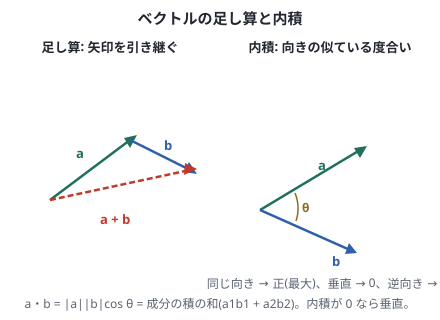
\includegraphics[width=0.9\textwidth]{figures/vector-basics.svg}
\caption{ベクトルの足し算と内積: 矢印の絵が計算の意味になる}
\end{figure}

\textbf{解答の指針:}\ ベクトルの問題では、まず\textbf{成分を書く}のが第一手です。絵だけ追っていると符号ミスが出ます。始点と終点の座標が与えられたら \( \vec{a} = \) 終点 − 始点 と成分に直し、長さ・平行(成分が比例)・中点(成分の平均)の判定はすべて成分で行います。絵に戻すのは最後の確認です。

\section{ベクトルの演算 — 足し算、実数倍、内積}

ベクトルの計算は、成分の世界では普通の算術です。\textbf{足し算は成分ごとの足し算}、\textbf{実数倍は成分ごとの掛け算}。

\[ (a_{1}, a_{2}) + (b_{1}, b_{2}) = (a_{1} + b_{1}, a_{2} + b_{2}) \qquad k(a_{1}, a_{2}) = (ka_{1}, ka_{2}) \]

絵での意味も対応させて覚えます。\textbf{足し算は「矢印を引き継ぐ」}(\( \vec{a} \) の終点から \( \vec{b} \) を描くと、始点から終点までが和)。\textbf{実数倍は矢印の伸縮}(\( k > 0 \) で同方向、\( k < 0 \) で逆方向)。

\subsection{内積: 向きの似ている度合いを 1 つの数に}

\textbf{内積}は、2 つのベクトルの向きの関係を 1 つの数にまとめたものです。

\[ \vec{a} \cdot \vec{b} = |\vec{a}||\vec{b}|\cos\theta \]

読み方の核心は\textbf{cos の部分}です。第 3 節で cos は「似ている向きの割合」を測る数だと見ました。2 つのベクトルが同じ向きなら cos = 1 で内積は最大、垂直なら cos = 0 で内積は 0、逆向きならマイナス。\textbf{内積 = 0 は垂直の条件}です。

成分でも計算できます。

\[ \vec{a} \cdot \vec{b} = a_{1}b_{1} + a_{2}b_{2} \]

この 2 通りの式が同じものを言っている、というのが内積の計算の中心です。左辺の形(長さと cos)から\textbf{幾何の意味}が読め、右辺の形(成分の積の和)から\textbf{計算の手順}が読めます。

\subsection{内積の使いどころ}

内積の応用は幅広いです。\textbf{垂直の判定}は内積 0。\textbf{なす角}は \( \cos\theta = \frac{\vec{a} \cdot \vec{b}}{|\vec{a}||\vec{b}|} \) から求める。\textbf{射影}(ベクトル \( \vec{b} \) が \( \vec{a} \) 方向にどれだけ伸びるか)も内積で計算でき、機械学習入門の主成分分析(線形代数応用編)の基礎の基礎です。物理の仕事(力 × 移動の向きに掛けた分)も、まさに内積でした(高校物理やり直し、エネルギーの節)。

\begin{quote}
\textbf{【注意】}\ 内積は「掛け算」ですが、\textbf{積の記号が点(・)である理由}は普通の掛け算と区別するためです。ベクトル同士の積には、内積のほかに「外積」(3 次元で使う別の積)がありますが、高校数学では内積だけです。内積の結果は\textbf{スカラー(数)}であってベクトルではない、という点も定番の確認事項です。
\end{quote}

\textbf{解答の指針:}\ 内積の問題では、(1) 2 つの式(幾何の形と成分の形)のどちらを使うかを選ぶ(長さと角度が分かっているなら幾何形、成分が分かっているなら成分形)、(2) 垂直の判定は内積 = 0、(3) なす角は cos に戻す、と手順を書きます。計算した内積が負になれば「逆向きに寄っている」と絵で確認するのが、符号ミスの最後の砦です。

\section{ベクトルと図形 — 絵を計算に、計算を絵に}

最後の節は、道具の総動員です。ベクトルの真の力は、\textbf{図形の関係(平行・垂直・点の位置)を方程式に翻訳できる}ことです。

\subsection{点の位置をベクトルで表す}

点 P が線分 AB を \( m : n \) に内分する点なら、位置ベクトルは次の式で書けます。

\[ \vec{p} = \frac{n\vec{a} + m\vec{b}}{m + n} \]

読み方は「\( m \) 倍寄りに重みを置いた平均」。中点は \( m = n \) の特別形(\( \frac{\vec{a} + \vec{b}}{2} \))です。\textbf{比の問題が、重み付き平均の式に翻訳できる}。図形の証明問題でベクトルが使われる理由の中心がここにあり、「点の位置」がすべて数で書けるようになります。

\subsection{証明の型: 平行と垂直を示す}

ベクトルによる図形の証明は、次の 2 つの型にほぼ集約されます。

\begin{itemize}
\item \textbf{平行を示す}: \( \vec{b} = k\vec{a} \) と書ける(成分が比例する)ことを示す。
\item \textbf{垂直を示す}: 内積が 0 になることを示す。
\end{itemize}

例えば三角形の三平方の定理(ピタゴラス)の証明も、辺をベクトルで書いて内積を展開すれば数行で終わります。幾何の補助線に頼らず、\textbf{手順として同じ計算}ができます。これは出題の傾向よりも深い話で、\textbf{機械学習や物理の計算がベクトルと内積で書かれている}のは、この「図形を自動的に計算できる」性質のためです。

\begin{quote}
\textbf{【注意】}\ ベクトルの証明で、図の形に頼った「見た目で分かる」は証明になりません。逆に、成分の計算だけを続けて絵を描かないと、結果の意味が分からなくなる。\textbf{最後に 1 度、絵に戻って確認する}のが、ベクトルを扱う上で最も大切な習慣です。
\end{quote}

\textbf{解答の指針:}\ ベクトルの図形問題では、(1) すべての点を位置ベクトルで書く、(2) 求めたい関係(平行なら比例、垂直なら内積 0)を式の形に翻訳する、(3) 計算して翻訳ミスがないか絵で確認する。内分点の問題は重み付き平均、中点はその特別形、と道具を割り当てます。「どの翻訳を使うか」を最初に 1 行書くのが、ベクトルの問題で迷わないコツです。

\section{まとめと次の一歩}

9 節を振り返ります。道具は、実は 4 つしかありません。

\begin{itemize}
\item \textbf{単位円}: 三角関数は円の上の点の座標。波と回転を結ぶ絵。
\item \textbf{加法定理}: 回転をまとめる式。倍角・半角はすべてここから導ける。
\item \textbf{図形と方程式}: 図形の条件を x と y の式に翻訳する。直線は傾きと 1 点、円は中心と半径。
\item \textbf{ベクトルと内積}: 幾何を成分の計算に翻訳する。垂直は内積 0、平行は比例。
\end{itemize}

数学の学習で一番効くのは、\textbf{絵と式の往復を自分で繰り返すこと}です。読んだ節のたびに、単位円・座標平面・矢印の絵を 1 枚手で描いてください。数学は「分かった気」になりやすい科目ですが、絵を描いて式を立てられるかどうかで理解の質が全く変わります。

次の一歩としては、この本の先は次のような本へつながります。

\begin{itemize}
\item ベクトルを行列・空間へ広げる → \textbf{大学数学入門}(線形代数の前半がその続きです)
\item 内積をデータ分析で使う → \textbf{線形代数 応用編}(主成分分析は内積の応用です)
\item sin の波を分解する → \textbf{フーリエ解析入門}(加法定理と積和の公式の先です)
\item 波の物理に戻る → \textbf{高校物理やり直し}(音と光の節と直接つながります)
\end{itemize}

この本で、中学数学 → 高校数学 → 大学数学の一本道がつながりました。まずは単位円を 1 枚描くことから始めてください。

\end{document}
